\documentclass[a4paper,11pt,fleqn]{scrartcl}%fleqn pour aligner les equations à gauche
\usepackage{../../Styles/Exercice}


\newcommand{\chnum}{Chapitre 8}
\newcommand{\chtitle}{Réaction chimiques forcées}
\newcommand{\dtype}{Exercices}


\begin{document}
	\maketitle
    \begin{multicols}{2}
\section{Schématiser les transferts d'électrons aux électrodes}
On considère l'électrolyse d'une solution d'acide sulfurique (\ce{2H+(aq) + SO4^2-(aq)}) au cours de laquelle on recueille du dihydrogène du côté de l'électrode B et du dioxygène du côté de l'électrode A.
\begin{data}
    Couples oxydant/réducteur mis en jeu : \ce{H+(aq)}/\ce{H2(g)} et \ce{O2(g)}/\ce{H2O(l)}
\end{data}
\begin{enumerate}
    \item Ecrire la demi-équation électronique de la réaction se produisant au niveau de chaque électrode.
    \item Compléter le schéma de l'électrolyse en précisant le sens de déplacement des électrons ainsi que les bornes du générateur.
\end{enumerate}
\begin{center}
    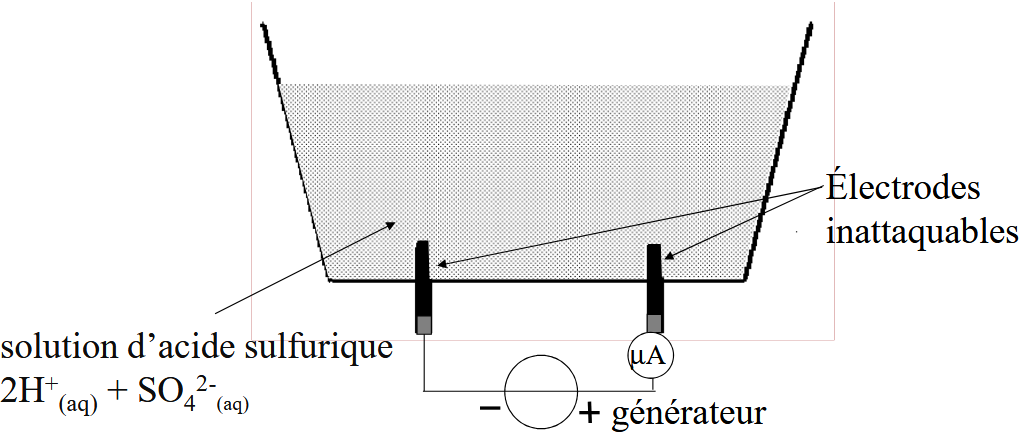
\includegraphics[width=.5\linewidth]{Ressources/TSPE_C08_Exercices_Fig1.png}
\end{center}

\section{Déterminer les variations de quantité de matière}
Un bijoutier souhaite donner plus d'éclat à une bague en or. Pour cela, il la recouvre de rhodium (un métal très brillant). Il réalise l'électrolyse d'une solution de nitrate de rhodium (\ce{Rh^3+(aq) + 3NO3-(aq)}) pendant 20 min en faisant circuler une intensité constante $I = \SI{0,40}{A}$.\\
On observe un dépôt de rhodium sur la bague, qui constitue la cathode, provenant de la réduction des ions rhodium (III) selon la demi-équation: \ce{Rh^3+ (aq) + 3e- = Rh (s)}\\
À l'anode, on observe un dégagement de dioxygène gazeux provenant de l'oxydation de l'eau selon la demi-équation:
$$\ce{2H2O(l) = O2(g) + 4H+(aq)+ 4e-}$$
\begin{data}
    Constante de Faraday : $\mathcal{F} =\SI{96500}{\coulomb\per\mole}$\\
    Masse molaire du rhodium : $M(\ce{Rh}) = \SI{102,9}{\gram\per\mole}$\\
    Volume molaire d'un gaz à \SI{20}{\celsius} et \SI{1013}{\hecto\pascal} : $V_m = \SI{24,0}{\mole\per\liter}$
\end{data}
\begin{enumerate}
    \item Calculer la quantité d'électricité $Q$ ayant traversé l'électrolyseur.
    \item En déduire la quantité de matière d'électrons échangés au cours de l'électrolyse.
    \item D'après les demi-équations, en déduire la quantité de matière de rhodium déposé sur la bague et la quantité de matière de dioxygène formé à l'anode.
    \item Déterminer la masse de rhodium déposé et le volume de dioxygène formé.
\end{enumerate}

\section{Nickelage électrolytique d'une pièce métallique}
Le nickel est un métal gris argenté qui possède une très bonne résistance à la corrosion. Pour réaliser le nickelage électrolytique d'un objet métallique, la solution à utiliser contient toujours des ions nickel de concentration habituellement de l'ordre de \SI{2}{\mole\per\meter}, il est préférable de maintenir cette concentration à peu près constante.
\begin{center}
    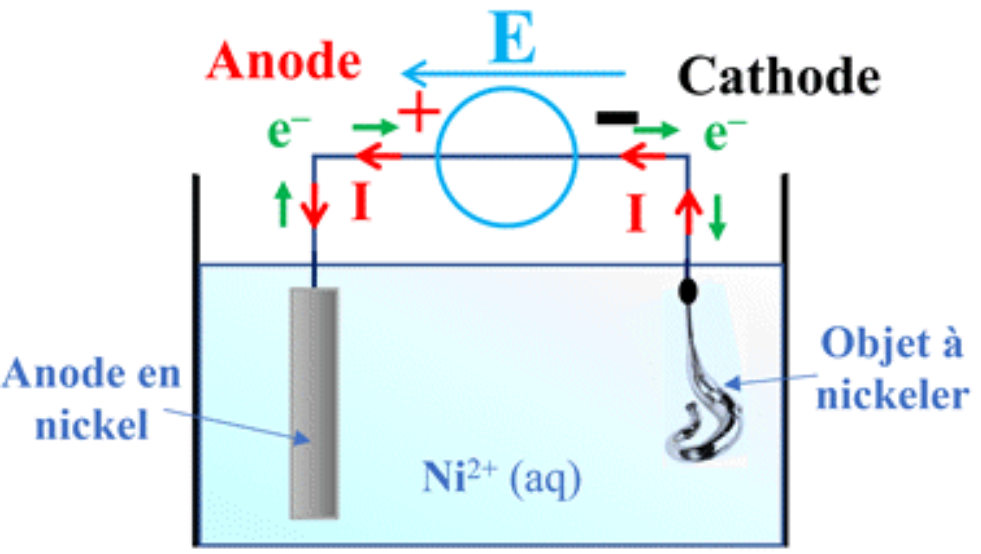
\includegraphics[width=.6\linewidth]{Ressources/TSPE_C08_Exercices_Fig2.png}
\end{center}

En pratique la pièce à nickeler, immergée dans le bain d'électrolyse contenant des ions \ce{Ni^2+}, est reliée au pôle négatif d'un générateur, alors que le pôle positif est relié à une électrode constituée de nickel pur comme le montre le schéma de la figure ci-dessus.
\begin{data}
    Masse molaire du nickel: $M(Ni) = \SI{59,0}{\gram\per\mole}$\\
    Couple mis en jeu: \ce{Ni^2+(aq)}/\ce{Ni(s)}\\
    Constante de Faraday : $\mathcal{F} =\SI{96500}{\coulomb\per\mole}$
\end{data}
\begin{enumerate}
    \item À quelle électrode faut-il brancher la pièce à nickeler ? Justifier en écrivant l'équation de la réaction modélisant la transformation qui a lieu sur cette pièce.
    \item La pièce constitue-t-elle l'anode ou la cathode de lélectrolyseur?
    \item Pourquoi l'électrode reliée à l'autre pôle du générateur est-elle en nickel?
    \item La masse de nickel à déposer sur la pièce est $m = \SI{3,0}{g}$. Déterminer la quantité de matière de nickel $n(\ce{Ni})$ correspondante, puis en déduire la quantité de matière d'électrons $n(\ce{e-})$ qui doit circuler pour permettre ce dépôt.
    \item L'intensité du courant utilisé est $I = \SI{8,0}{A}$. Calculer la durée $\Delta t$ nécessaire à l'électrolyse.
\end{enumerate}
\end{multicols}
\end{document}